
%%%%%%%%%%%%%%%%%%%%%%% file typeinst.tex %%%%%%%%%%%%%%%%%%%%%%%%%
%
% This is the LaTeX source for the instructions to authors using
% the LaTeX document class 'llncs.cls' for contributions to
% the Lecture Notes in Computer Sciences series.
% http://www.springer.com/lncs       Springer Heidelberg 2006/05/04
%
% It may be used as a template for your own input - copy it
% to a new file with a new name and use it as the basis
% for your article.
%
% NB: the document class 'llncs' has its own and detailed documentation, see
% ftp://ftp.springer.de/data/pubftp/pub/tex/latex/llncs/latex2e/llncsdoc.pdf
%
%%%%%%%%%%%%%%%%%%%%%%%%%%%%%%%%%%%%%%%%%%%%%%%%%%%%%%%%%%%%%%%%%%%


\documentclass[runningheads]{llncs}

\usepackage{amssymb}
\setcounter{tocdepth}{3}
\usepackage{graphicx}
\usepackage{hyperref}
\usepackage{url}
\usepackage[english]{babel}
\usepackage{graphicx}
\urldef{\mailsa}\path|{aysengupta, xianlin, ksanjeev, sravichandra}@cs.stonybrook.edu|
\newcommand{\keywords}[1]{\par\addvspace\baselineskip
\noindent\keywordname\enspace\ignorespaces#1}
\newcommand{\swallow}[1]{ }

\begin{document}

\mainmatter  % start of an individual contribution

% first the title is needed
\title{Final Report: Team 8\\
Predicting Prices of Oil and Gold}

% a short form should be given in case it is too long for the running head
\titlerunning{Predicting the Prices of Oil and Gold}

% the name(s) of the author(s) follow(s) next
%
% NB: Chinese authors should write their first names(s) in front of
% their surnames. This ensures that the names appear correctly in
% the running heads and the author index.
%
\author{Ayush Sengupta \and Benjamin Lin \and Komal Sanjeev \and Sreevathsan Ravichandran}
%
\authorrunning{Ayush Sengupta \and Benjamin Lin \and Komal Sanjeev \and 	vathsan Ravichandran}
% (feature abused for this document to repeat the title also on left hand pages)

% the affiliations are given next; don't give your e-mail address
% unless you accept that it will be published
\institute{Department of Computer Science, Stony Brook University,\\
Stony Brook, NY 11794-4400\\
\mailsa\\
\url{http://www.cs.stonybrook.edu/~skiena/591/projects}}

%
% NB: a more complex sample for affiliations and the mapping to the
% corresponding authors can be found in the file "llncs.dem"
% (search for the string "\mainmatter" where a contribution starts).
% "llncs.dem" accompanies the document class "llncs.cls".
%

\toctitle{Lecture Notes in Computer Science}
\tocauthor{Authors' Instructions}
\maketitle

\swallow{   % DO NOT BOTHER WITH THIS
\begin{abstract}
The abstract should summarize the contents of the paper and should
contain at least 70 and at most 150 words. It should be written using the
\emph{abstract} environment.
\keywords{We would like to encourage you to list your keywords within
the abstract section}
\end{abstract}
}


\section{Challenge} 

Our challenge is to predict the prices of Oil and Gold on January 1st 2015 as of December 1st in 2014 (a month in advance). \\

\noindent Oil and Gold are extensively traded commodities, and there are several macroeconomic factors which affect the prices, thus causing the prices of these commodities to be extremely volatile. Certain factors are also interdependent, which makes it extremely difficult to estimate the extent to which an individual factor could affect the price of a commodity. Moreover, the relationship between the factors and the prices could also vary over time. This makes the prediction of oil and gold prices a very complex and challenging problem.


\subsection{Oil}

Oil is a non-renewable resource which occurs in the earth. It is extracted and sent to refineries where different petroleum products such as gasoline, petrol, heating oil, etc are separated. Almost two-thirds of our energy demands are met by oil. Oil is the most heavily and actively traded commodity, which accounts to almost 10\% of the world's trade.\\

\noindent The price of oil is determined by supply and demand. An increase in demand results in an increase in the price of oil, and vice versa. The supply and demand themselves are determined by various factors such as economy, weather and geopolitics. \\

\noindent 
\subsection{Gold}
Gold has been viewed as a symbol of wealth since the ancient times of the human history. It is widely used as jewellery and in some precision gauges. \\

\noindent For a long period of time, the price of gold was fixed. After 1968, with the breakdown of the Bretton Woods Currency Arrangement, the price of gold began to be determined by the market. Gold is also used as an investment to hedge against market fluctuations. 


\section{History/Background}
\subsection{Factors Affecting the Price of Oil}
Crude oil prices are determined by the balance between supply and demand. An increase (or decrease) in demand causes the price of oil to rise (or fall). Consequently, a cutback in the supply of oil results in an increase in oil prices. There are several factors which disturb the supply-demand balance, thus resulting in oil price fluctuations. 


\begin{figure}
\centering
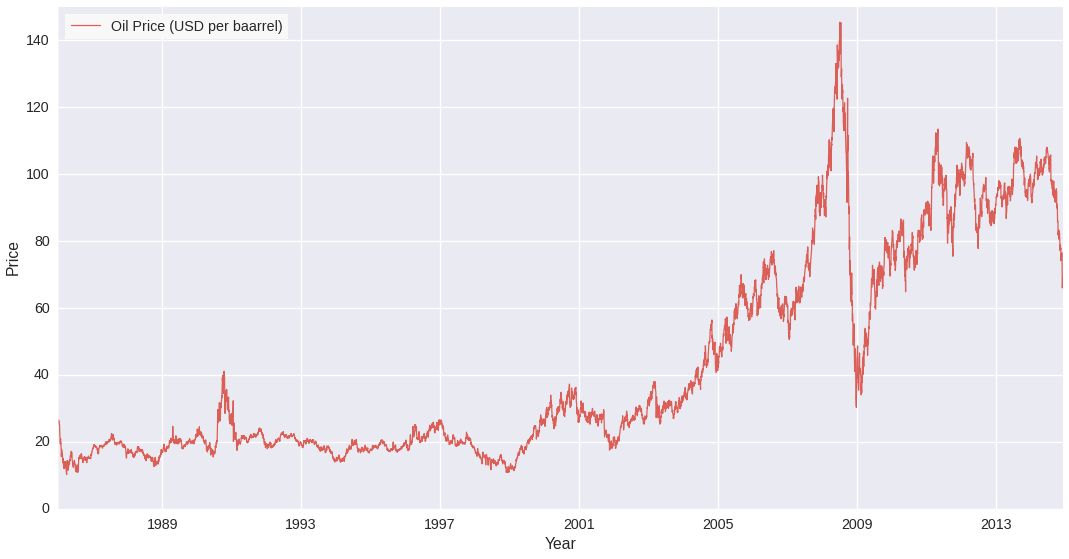
\includegraphics[width=\textwidth]{Oil_since1970.png}
\caption{Historical Oil Prices - US Dollar per Barrel - 1986 to 2014}
\label{fig:Oil_since1970.png}
\end{figure}

\subsubsection{Organization of the Petroleum Exporting Countries (OPEC) Supply}
OPEC is an organization of 12 oil exporting nations, namely Algeria, Angola, Ecuador, Iran, Iraq, Kuwait, Libya, Nigeria, Qatar, Saudi Arabia, United Arab Emirates, and Venezuela. It aims at coordinating and unifying petroleum prices of its member countries \cite{opec}.Oil supply from the OPEC member countries represents about 40\% of the world’s crude oil, and their actions can affect the prices of oil to a significant extent. For example, limiting the oil production from OPEC’s major oil producers such as Saudi Arabia can influence crude oil supply and affect the prices \cite{eiafactors}.\\ 
\noindent Oil prices not only depend on the current demand and supply, but also on the projected future supply and demand. OPEC adjusts the oil productions of its member countries based on current and future demand.

\subsubsection{Non-OPEC Supply}
The non-OPEC countries produce about 60\% of the world's crude oil. A reduction of supply from the non-OPEC countries creates additional pressure on the OPEC countries, which can also contribute to a rise in oil prices \cite{eiafactors}.

\subsubsection{Stock Market}
The stock market can be used as an indicator of the economy. As economic conditions improve, there is an increase in demand for several commodities including oil, which results in an increase in oil prices. The Standard and Poor's 500 (S\&P 500) index is a common benchmark for the stock market of USA. It is a weighted index of the market capitalization of 500 companies. It is the most commonly used indicator of the US economy.

\subsubsection{Seasonal Effects}
Certain crude oil products such as heating oil and gasoline tend to have a seasonal variance. For example, there is an increase in demand for oil in the fourth quarter due to the cold weather, and a subsequent reduction in demand during late winter as the weather gets warmer. Gasoline prices also tend to rise in the summer due to an increased consumption. 

\subsubsection{US Dollar}
Oil is traded in Dollars, and hence, any change in the strength of the Dollar relative to other currencies can cause oil prices to shift. The US Dollar Index is a measure of the United States Dollar relative to a basket of foreign currencies. Several studies support the negative correlation between the US Dollar Index and the price of oil. There are several arguments to support this statement. One reason could be that the depreciation in the dollar exchange rate causes oil to be cheaper in countries outside the US, thus leading to an increase in demand, which in turn causes oil prices to rise. However, it has been observed that the relationship between oil prices and the dollar exchange rate has not been stable over the years \cite{eiafactors} \cite{oildollar}.

\subsection{Factors Affecting the Price of Gold}
Gold is a precious metal which was used as a currency in several major civilizations in the past centuries. In the Unites States of America, gold had been at a fixed price of about \$20 per ounce, since the early 19th century. In 1934, President Franklin Roosevelt raised gold price from \$20.67 per ounce to \$35. In 1968, with the breakdown of Bretton Woods Currency Arrangements, the gold price became market determined. From \autoref{fig:Gold_since1970.png} below, we observe that the two peaks of the gold price coincide with two significant economic recessions in our history - one in 1980, and the other 2008.\\

\begin{figure}
\centering
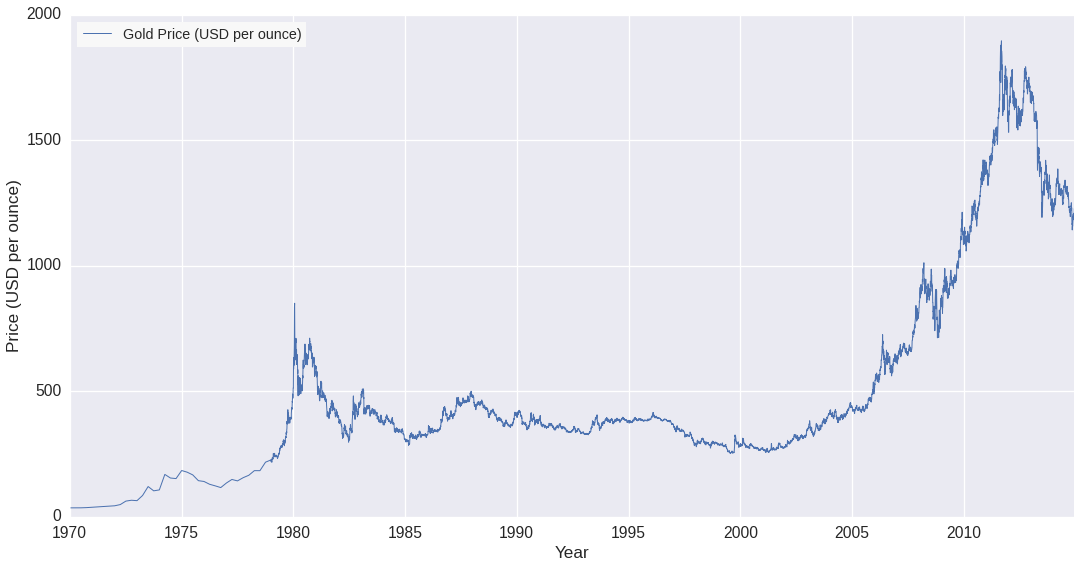
\includegraphics[width=\textwidth]{Gold_since1970.png}
\caption{Historical Gold Prices - US Dollars per ounce from Jan 1, 1970 to Dec 9, 2014}
\label{fig:Gold_since1970.png}
\end{figure}

\noindent The price of gold is determined by several factors, the most significant being, Crude Oil Price, Commodity Research Bureau Future Index (CRB), EURO/USD Exchange Rate (EURO/USD), Inflation Rate (INF), Money Supply (M1), and the US Dollar Index (USDX) \cite{gold-shafiee}\cite{gold-zhang}\cite{gold-Ismail}. 

\subsubsection{Consumer Sentiment Index (CSI)} 
The Consumer Sentiment Index or Consumer Confidence Index, is an index measuring the consumers' confidence over the market \cite{csi-1}\cite{csi-2}. Similar to the effects of USDX over the gold price, a high CSI indicates consumers generally feel optimistic about the overall economy and their ability of obtaining and keeping their jobs, so they would be less likely to keep precious metals like gold.

\subsubsection{Crude Oil Price}
Crude oil prices are highly correlated to gold prices. Rising oil prices may lead to an increase in the gold price, but the converse may not be true \cite{gold-shafiee}\cite{gold-zhang}.
The gold-oil relation suggests that the crude oil price could partly account for inflation. An increase in the oil price results in increased prices of gasoline. Gasoline being more expensive results in an increase in the cost to transport goods, thus causing a possible hike in prices of goods. The final result is an increased price level – in other words, inflation. Gold tends to appreciate with inflation. Therefore, elevated oil prices can eventually lead to higher gold prices \cite{gold-url1}. 

\begin{figure}
\centering
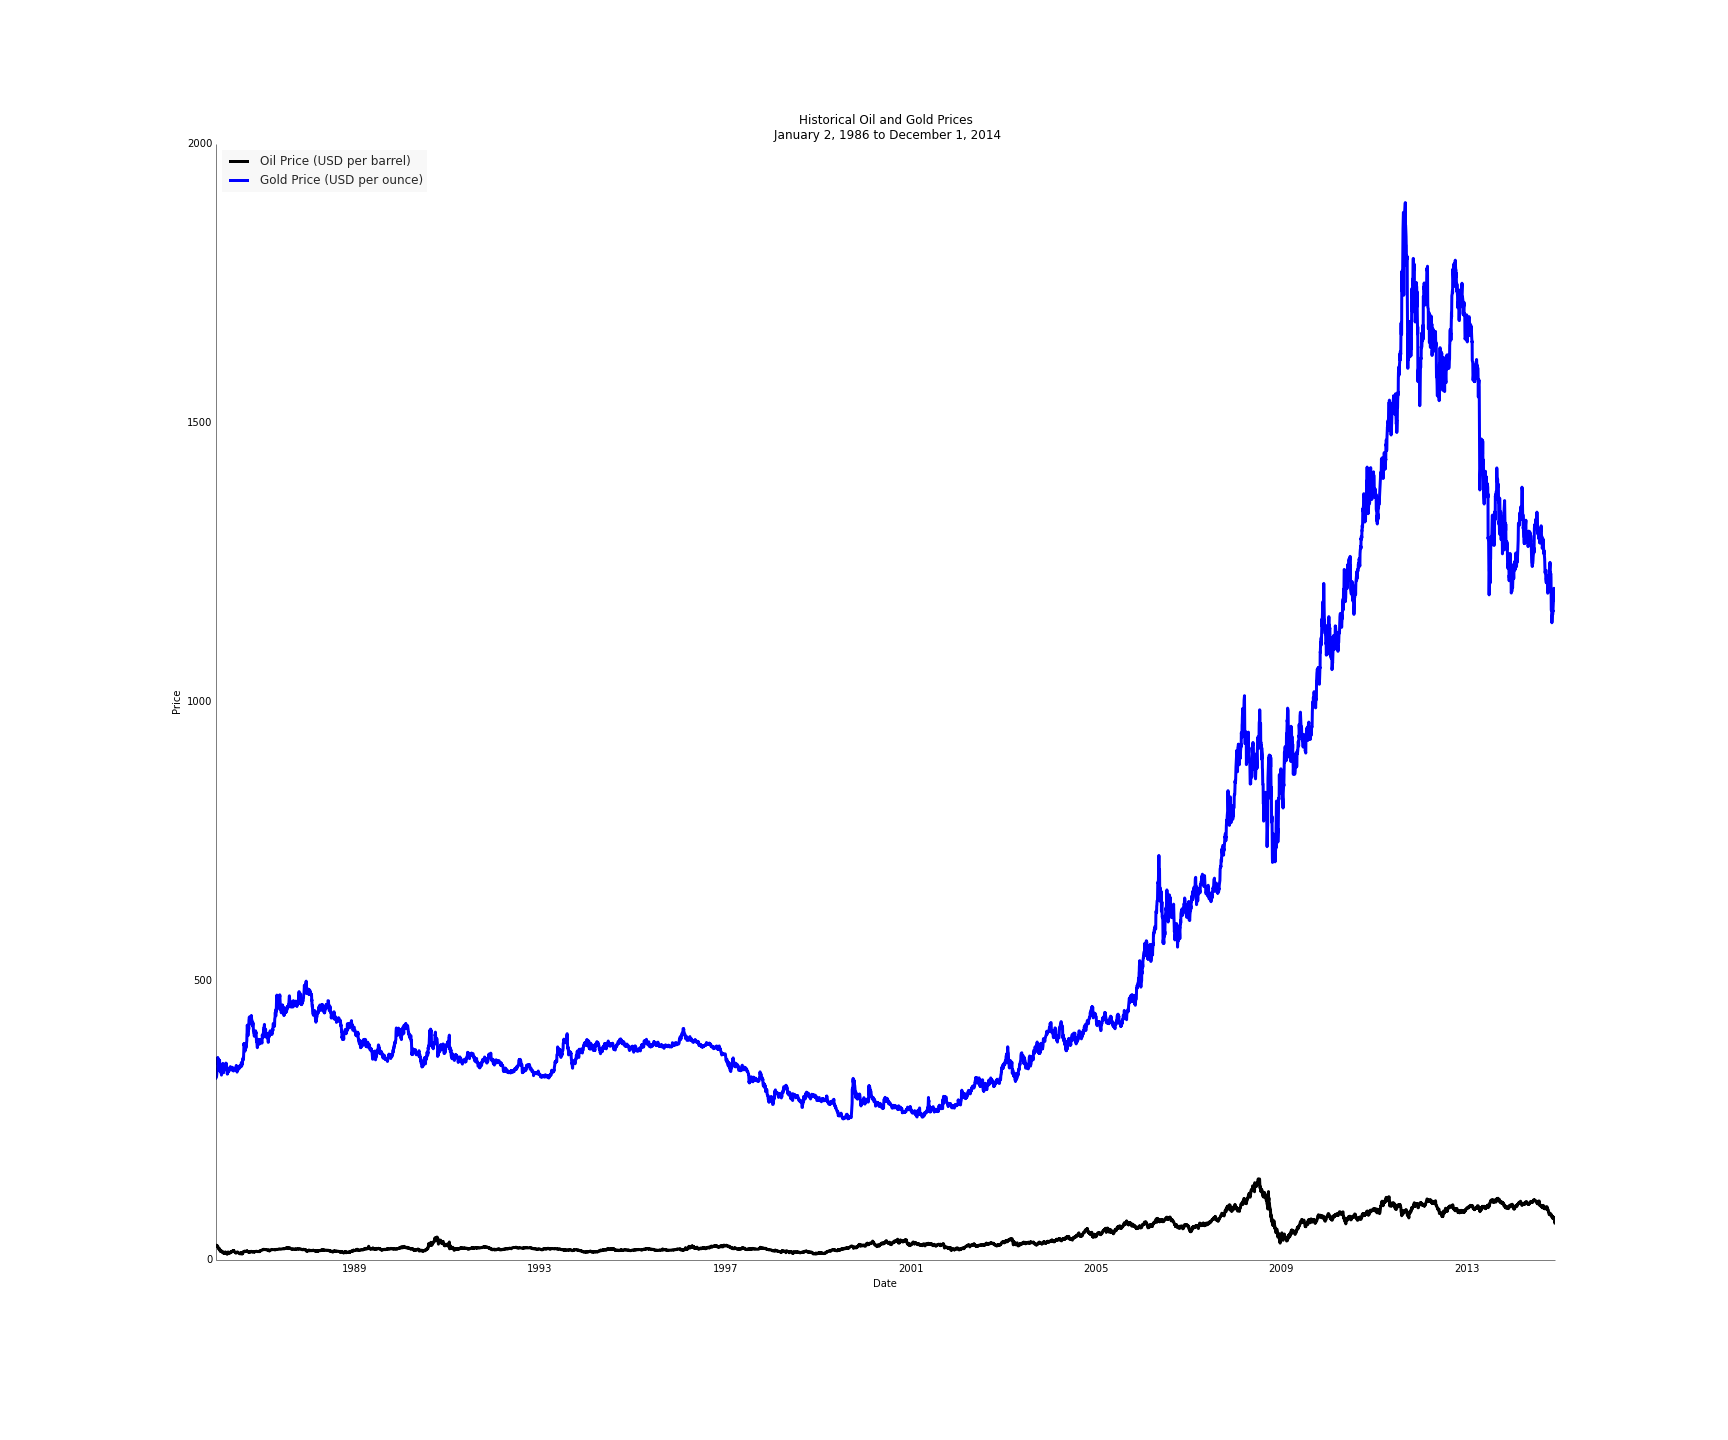
\includegraphics[width=\textwidth]{OilvsGold.png}
\caption{Historical Oil and Gold Prices showing correlation}
\label{fig:OilvsGold.png}
\end{figure}

\newpage

\subsection {Futures Contracts}

\noindent A forward or a futures contract is an agreement to buy or sell an asset at a certain time in the future for a certain price. Two parties are involved in a futures contract, where one assumes a long position and agrees to buy the asset for a specific price at a particular time, and the other assumes a short position, and agrees to sell the same asset at the same price and time. \\

\noindent Futures contracts can be used to hedge market risks. Consider the current price of crude oil to be $\$70$ a barrel, and an individual speculates that the price is going to increase in the future, he can enter a long contract to purchase 100 barrels of crude oil at $\$70$ a barrel on a date 3 months from now. If the price of oil does increase to say $\$75$ a barrel, the individual benefits because he pays only $\$70$.\\

\noindent Futures contracts are also used by speculators to make profits. Suppose an individual enters a short contract to buy 100 barrels of oil at $\$70$ a barrel on April 1 2015. The price of the contract is $\$7000$. If the price of crude oil rises to $\$72$ a barrel on March 1 2015, he can sell the contract early for $\$7200$, thus making a profit of $\$200$. \\

\noindent The prices of futures contracts are determined by the supply and demand. If there are more sellers than buyers, the prices go down. If more traders wish to buy the commodity rather than sell, the prices goes up. As the delivery period for a futures contract is approached, the futures price converges to the spot price. For example, consider that the current price of a futures contract is higher than the spot price. In such a scenario, more individuals will be willing to go short and sell contracts, thus increasing the supply and causing the price to decrease and eventually converge to the spot price. The converse is also true when the price of the futures contract is lesser than the spot price. More individuals will be interested in buying contracts, this increasing the demand, and consequently the price of the contracts. \\
 
\noindent The prices of these contracts constantly change in response to newly obtained information in the market. Information can be obtained from various sources, for example, the US Energy Information Administration (EIA) provides weekly data of crude oil supply. This newly obtained information affects the prices of the underlying crude oil futures contracts. \\

\noindent These futures contracts encapsulate information about future trends, because they contains collective information of what several individuals think about the future market trends. Several experts claim that the spot prices hold as much information as the futures prices, and are equally good estimators of the future trends. 

\newpage

\section{Literature Review}
A significant amount of research has been done to understand and predict oil and gold prices. Various studies have developed different predictive models based on different techniques and factors. Some studies try to make predictions based on historical oil and gold prices. Others focus on the economic aspects and try to explain the correlations between the prices of oil and gold with respect to a variety of economic factors. Therefore, we evaluate and summarize some widely used models into the following two categories: Standard Time Series Models and Structural Models Considering Economic Factors.

\subsection{Standard Time Series Models(Technical Models)}
Standard time series models attempt to predict the oil price using the current and historical oil prices. The same strategy applies to predicting the gold price as well. These models are useful in the following scenarios:
\begin {itemize}
\item The prices show autocorrelation and autoregressive behavior, i.e., there is a pattern or a significant correlation between current and the previous prices.\\
\item There are a large number of explanatory variables and it is difficult to understand them well because they interact with each other in a very complicated manner. \\
\item Forecasting the dependent variable may require predicting the explanatory variables. And prediction of the explanatory variable might in turn be a harder problem.\\
\item Not all explanatory factors and variables are known.\\ 
\end {itemize}


\noindent The most basic time series models that have been applied to model oil prices are the autoregressive models. In general, an autoregressive model \textbf{AR(p)} tries to model the current value of a time series based on the value of the last 'p' instances in the time series.\\

\noindent Thus, $ X_{t} = c + \sum\limits_{i=1}^p \varphi_{t-i}X_{t-i} + \epsilon_{t}$.\\\\

\noindent The co-efficients are regressed to predict the current price. Here the term $\epsilon_{t}$ is known as the \textit{white noise}. It is a random variable with zero mean, constant variance. Also, $corr(\epsilon_t,\epsilon_{t-1})$ is $0$ $\forall i>1$ and it is $1$ for $i=0$. In other words, $\epsilon_{t}$ is a random variable with no auto-correlation.\\

\noindent Similarly, Autoregressive Moving Average (ARMA) models take in to account the moving average factor. They try to predict the randomness based on the historical prices.  Hence \textbf{ARMA(p,q)} can be written as:\\

$ X_{t} = c + \sum\limits_{i=1}^p \varphi_{t-i}X_{t-i} + \epsilon_{t} + \sum\limits_{i=1}^q \theta_{t-i}\epsilon_{t-i}$.\\
\\

\noindent Further, it is known that oil price changes(volatility) follow GARCH/ARCH properties. Least square models generally assume that the expected value of all error terms, when squared, is constant. This assumption is termed as homoskedasticity. Data(time series) in which this conditions fail to hold, are heteroskedastic. ARCH and GARCH models treat heteroskedasticity as a variance which is then modelled autoregressively.\cite{engle}\\

\noindent In short, GARCH models split the error-terms $\varepsilon_t$ into a stochastic component $z_{t}$ and a time dependent variance $\sigma^2_{t}$. Thus, $ \varepsilon_t = z_{t} + \sigma_{t}$. The series $\sigma^2_{t}$ in \textbf{ARCH(q)} is modelled by:\\\\

$\sigma^2_{t} = \alpha_{0} + \sum\limits_{i=1}^q \alpha_{i}\varepsilon_{t-i}^2 $\\\\

\noindent Similarly \textbf{GARCH(p,q)} is modelled by:\\\\

$\sigma^2_{t} = \alpha_{0} + \sum\limits_{i=1}^q \alpha_{i}\varepsilon_{t-i}^2 + \sum\limits_{i=1}^p \beta_{i}\sigma_{t-i}^2 $\\\\

\noindent GARCH and ARCH models have consistently been used in the literature to predict oil prices with varying degrees of accuracy. 

\subsection{Structural Models Considering Economic Factors}

For the price of oil, structural models consider the oil price to be modelled as a function of certain explanatory variables such as oil consumption and production, OPEC behaviour, interest rates, exchange rates, and other commodity prices. The major drawback of using structural models to predict oil prices is that the models are extremely complex, and there is a strong inter correlation between factors themselves. Hence, there have not been many studies that focus on structural analysis to forecast oil prices.\\

\noindent According to Huntington(1994)\cite{huntington}, structural demand and supply models are generally not successful in predicting oil prices due to inaccurate forecasts of GDP and the oil supply from different countries. Another reason was not taking into account the market participation expectation of OPEC countries. \\

\noindent However, some interesting work has been done based solely on structural models. Most of these studies use models and results that instead of trying to predict the price, try to understand the nature of the oil market. Also, these models predict short-term oil prices, and it is unclear if they could be used for long term forecasting. One such interesting study by Pindyck(1999)\cite{pindyck} shows that long term oil prices are mean reverting around shifting trend lines. \\

\noindent In another direction Yang et al.(2002) \cite{yang} introduces a model to determine the factors affecting US oil prices. First, they highlight the unstable demand structure of the oil market. Then, they use a GARCH model (general autoregressive conditional heteroskedasticity) to investigate the volatility of oil prices. Using the co-efficients they generated, they estimate that the future oil price will be $0.987$ times the current oil price if the US GDP decreases by $5\%$. \\

\noindent Similarly, structural models considering a variety of economic factors also apply to the gold price prediction. According to Ismail et al.(2009)\cite{gold-Ismail}, they design models with the gold price as the only dependent variable, alongside different numbers of independent variables. Initially, they propose that the gold price is dependent on the following 8 factors: Commodity Research Bureau future index (CRB), USD/Euro Foreign Exchange Rate (EUROUSD); Inflation rate (INF); Money Supply (M1); New York Stock Exchange (NYSE); Standard and Poor 500 (SPX); Treasury Bill (T-BILL) and US Dollar index (USDX). Therefore, their first-order regression model, which they call it naive model, is like: \\

$\hat{Y}=-560.618+0.712X_1+161.740X_2-7.836X_3 +0.424X_4-0.010X_5+0.010X_6+3.198X_7+0.580X_8$ \\\\
where $\hat{Y}$ is the predicted gold price; $X_1$ is CRB; $X_2$ is EUROUSD; $X_3$ is INF; $X_4$ is M1; $X_5$ is NYSE; $X_6$ is SPX; $X_7$ is T-Bill; $X_8$ is USDX.\\

\noindent Then they show that using stepwise regression, the number of independent variables can be reduced from 8 to 4. Their enhanced model is  \\

$\hat{Y}=-301.509+0.676X_1+114.651X_2-5.563X_3+0.309X_4$ \\\\
where $\hat{Y}$ is the predicted gold price, $X_1$ is CRB; $X_2$ is EUROUSD; $X_3$ is INF; $X_4$ is M1. \\

\noindent Ismail's paper provides us the intuition of what factors we may use for building our own advanced models (autoregressive and multiple linear regression models) in predicting the gold price. In our advanced models, we include the S\&P 500 Index, NYSE Index and the US Dollar Index that are mentioned in Ismail's paper, as well as Consumer Sentiment Index and the oil price that are not. The details will be discussed in Section 7 "Advanced Models".\\

\subsection{Non Standard Models}

\noindent Non standard methods have gained popularity because most of the linear time series model fail to take into account the non-linearity of the data. Oil prices and gold prices have a strong non-linear and chaotic time series and some experts think that non-linear models might fit quite well in this context.\\\\
\noindent Several non stanmdard and non-linear methods have been applied to the time series in recent times. One such interesting method is the Emperical Mode(EMD) Decomposition method\cite{oil-zhang}. This paper assumes that the data. depending on its complexity, may have several different co-existing modes of oscillations. The authors try to extract these modes of oscillation and then they add them to forecast oil prices. EMD is a relatively innovative approach for modelling time series data and they seem to give relatively good results for long term predictions.\\\\
\noindent Support Vector Machines have also gained popularity for oil price forecasting. These methods have been used for forecasting oil consumption as well. For example, Dong et al(2005)\cite{dongbing} have used it to forecast oil consumption in tropical regions. Lin and Pai(2004) have tried to use a hybrid model of Support Vector Machines and ARIMA model to model oil prices. Here the ARIMA models the linear aspects of the time series, whereas the SVM tries to model the non-linear aspects. They evaluated their results based on real data and seem to get very positive results.\\\\
\noindent Another interesting tool being used in recent time s for oil price forecasting(and stock price predictions in general) is Artificial Neural Networks. ANNs are computational models inspired by the central nervous system and are used to estimate functions that can depend on large number of unknown inputs. Multiple ANN approaches have been used to predict oil prices and they all achieve varying degrees of accuracy. One interesting hybrid ANN as well as regression approach is the NARX(non linear autoregressive model with eXogenous input) model. They claim that the NARX model is more accurate than time series and static ANN models in predicting oil prices in general as well as in predicting the occurence of oil price shocks.\\\\
   

\newpage

\section{Data Sets}

\noindent Our data consists of multiple time series of monthly Oil and Gold prices \cite{quandal}, and related macroeconomic factors.\\

\noindent Crude oil benchmarks are reference prices for buyers and sellers. There are several benchmarks for the prices of oil, out of which the most popular ones are West Texas Intermediate (WTI), Brent, Dubai. 
Spot Price is the current price at which a particular security can be bought or sold at a specified time and place. 
Historical WTI Crude Oil prices and spot prices of gold were used for making predictions.

\begin{figure}
\centering
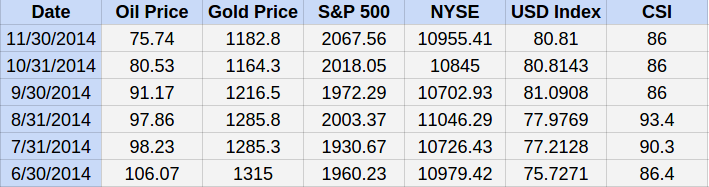
\includegraphics[width=\textwidth]{DataMatrices.png}
\caption{Data matrix for oil and gold price and its related macroeconomic factors}
\label{fig:DataMatrices.png}
\end{figure}

The following macroeconomic factors were used:

\begin {itemize}
\item S\&P 500 Index \cite{quandal}
\item New York Stock Exchange Index (NYSE) \cite{quandal}
\item US Dollar Index \cite{quandal}
\item Consumer Sentiment Index (CSI) \cite{csi}
\end {itemize}


\noindent The aforementioned data sets are monetary time series, and it is important to adjust for inflation in order to eliminate the unnecessary correlation caused due to inflation. Inflation adjustment is done by dividing the monetary time series by a price index, which is a number representing the price level relative to a base year. The Consumer Price Index (CPI) was used to adjust for inflation.

\newpage

\section{Observations}

\noindent The correlation matrices in \autoref{fig:Correlation_Oil_Value_.png} and \autoref{fig:Correlation_Gold_Value_.png}, show the correlation between the price of oil/gold and related economic factors. \\

\begin{figure}
\centering
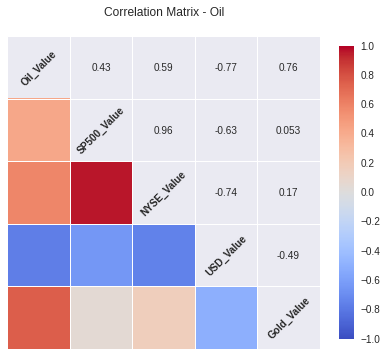
\includegraphics[width=\textwidth]{Correlation_Oil_Value_.png}
\caption{Correlation Matrix for Oil Price and related macroeconomic factors}
\label{fig:Correlation_Oil_Value_.png}
\end{figure}

\begin{figure}
\centering
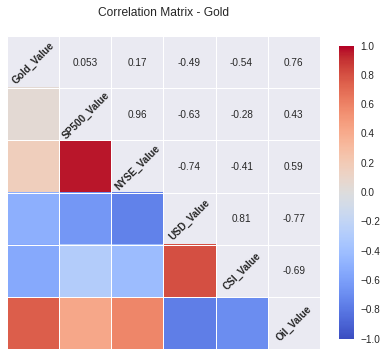
\includegraphics[width=\textwidth]{Correlation_Gold_Value_.png}
\caption{Correlation Heat Map for Gold Price and related macroeconomic factors}
\label{fig:Correlation_Gold_Value_.png}
\end{figure}

\newpage

\section{Baseline Models}
We initially developed very simple baseline models which predict the price as a simple function of the past few months. In order to illustrate an improvement in the accuracy of our predictions, we compare our advanced models to the following baseline models:

\begin {itemize}
\item \textbf{Baseline Model 1} The price is the same as the previous month's price: \\
$P_{t}$ = $P_{t-1}$\\
\item \textbf{Baseline Model 2} The price is a cubic weighted average of the last 3 months: \\
$P_{t}$ = $\frac{1}{\{k(k+1)\}^2}\sum\limits_{i=1}^k (k-i+1)^3P_{t-i}$
\end {itemize}

\section{Advanced Models}

We developed autoregressive models, autoregressive models with multiple linear regression to incorporate macroeconomic factors, and regression models using futures data to make our predictions. \\

\subsection{Autoregressive Models}
\noindent\textbf{Autoregressive Model} This model is purely based on the historical prices. It models the time series as a linear function of the values of the past 'p' months.\\

$ X_{t} = c + \sum\limits_{i=1}^p \varphi_{t-i}X_{t-i}$. \\

\noindent The Ordinary Least Squares (OLS) method is used to estimate the parameters of the regression function. It tries to minimize the sum of squares of vertical distances between the predicted and the actual values. \\

\noindent\textbf{Autoregressive Moving Average} ARMA models are used to understand and predict time series values as a function of two polynomials, an autoregressive function, and a moving average function. 
\\

$ X_{t} = c + \sum\limits_{i=1}^p \varphi_{t-i}X_{t-i} + \epsilon_{t} + \sum\limits_{i=1}^q \theta_{t-i}\epsilon_{t-i}$.\\\\

\noindent Here $\epsilon_t$ is the random white noise, a random variable with zero mean, constant variance and zero auto-correlation.

\noindent In ARMA (p,q), p is referred to as the order of the autoregressive part and q is referred to as the order of the moving average part, i.e, the model is described using p autoregressive terms and q moving average terms.\\ 

\subsection{Autoregressive and Multiple Linear Regressive Models Considering Macroeconomic Factors}
Linear regression models the relationship between two variables - a dependent variable and an explanatory variable using a linear function. The process of modelling a variable based on more than one explanatory variables is called Multiple Linear Regression. \\
   
\noindent The pure autoregressive model was expanded to incorporate the macroeconomic factors which are highly correlated to the price of commodity being predicted. As the various factors are incorporated into the model, a comparison of the error metrics is performed to estimate the set of macroeconomic factors which make predictions with the best accuracy. \\


\noindent For predicting the price of oil, the following macroeconomic factors are taken into consideration:
\begin {itemize}
\item S\&P 500 Index
\item NYSE Index
\item US Dollar Index
\item Gold Price
\end {itemize}

\noindent For predicting the price of gold, the following factors macroeconomic are taken into consideration:
\begin {itemize}
\item S\&P 500 Index
\item NYSE Index
\item US Dollar Index
\item Consumer Sentiment Index
\item Oil Price
\end {itemize}

\subsection{Regression using Futures Data Models}

\subsubsection{Futures Model 1}
Past futures prices are used to predict the current spot price. A simple regression is used to make predictions. This model can be represented as follows:\\

$X_t = \sum\limits_{i=1}^k \alpha_{i}F_{t-i}^t + c$.\\

\subsubsection{Futures Model 2}
\noindent The Futures Model 1 is improved, and instead of trying to predict the spot price, we try to predict the difference in the current spot price and the last months spot price, using the difference in the futures price at lag $i$ and the spot price at lag $i$. This model can be represented as follows:\\

$X_t - X_{t-1} = \sum\limits_{i=1}^k \beta_i(F_{t-i}^t - X_{t-i}) +c$.


\subsection{Evaluation}

\noindent The models are trained on the initial 70\% of the time series, and tested on the remaining 30\%. They try to generate a linear function while assigning coefficients to each of the parameters. These regression coefficients are then used to make predictions. \\

The performance of our models is evaluated based on the following error mertics:

\begin {itemize}

\item \textbf{Mean Relative Error (MRE)}\\
$MRE = \frac{1}{n}\sum\limits_{i=1}^n \frac{|P^*_{t} - P_{t}|}{P_t}$\\

\item \textbf{Mean absolute Error (MAE)}\\
$MAE = \frac{1}{n}\sum\limits_{i=1}^n |P^*_{t} - P_{t}|$\\

\item \textbf{Root Mean Square Error (RMSE)}\\
$RMSE = \frac{1}{n}\sqrt{\sum\limits_{i=1}^n (P^*_{t} - P_{t})^2}$\\

\end {itemize}

A histogram of the distribution of relative error is also generated.

\subsection{Performance of Models Predicting the Price of Oil}

\noindent The following is a comparison of the performance all the models used for predicting the price of oil.

\begin{table}
\begin{center}
\begin{tabular}{|c|c|c|c|c|c}
\hline
\textbf{Model} & \textbf{Mean Rel Error} & \textbf{Mean Abs Error} & \textbf{RMSE} \\ \hline \hline$ Baseline\ 1\- Price\ Remains\ Same$ & $6.58\%$ & $5.93$ & $7.85$ \\ \hline
$ Baseline\ 2\ - Price\ is\ a\ Weighted\ Average$ & $7.17\%$ & $6.37$ & $8.58$ \\ \hline\hline
$ Autoregressive\ Model $ & $7.36\%$ & $5.73$ & $7.29$\\ \hline
$ Autoregressive\ Moving\ Average\ Model $ & $6.78\%$ & $5.03$ & $5.42$ \\ \hline\hline
$ Autoregressive\ - factors:\ Gold $ & $7.27\%$ & $5.67$ & $7.21$ \\ \hline
$ Autoregressive\ - factors:\ SP500,\ Gold $ & $6.99\%$ & $5.52$ & $7.16$ \\ \hline
$ Autoregressive\ - factors:\ NYSE,\ Gold $ & $7.06\%$ & $5.56$ & $7.16$ \\ \hline
$ Autoregressive\ - factors:\ NYSE,\ USD,\ Gold $ & $7.17\%$ & $5.61$ & $7.14$ \\ \hline
$ Autoregressive\ - factors:\ SP500,\ USD,\ Gold $ & $7.04\%$ & $5.54$ & $7.12$ \\ \hline\hline
$ Futures\ Prices\ Model\ 1 $ & $3.75\%$ & $3.80$ & $4.41$ \\ \hline
$ Futures\ Prices\ Model\ 2 $ & $3.03\%$ & $3.63$ & $4.32$ \\ \hline
\end{tabular}
\end{center} 
\caption{Error Metrics of various models for predicting the price of oil}
\end{table} 


\autoref{fig:ModelComparison_Oil.png} shows the comparison of the relative errors of different predictive models. \autoref{fig:OilErrorHistogram.png} shows the error histograms generated by different models.


\subsubsection{Summary}

\begin {itemize}

\item Among the autoregressive models, ARMA performed the best with a Mean Relative Error of 6.78\%. \\
\item Among the regressive models considering economic factors, the model considerting S\&P 500 and the Gold Price performed best with a Mean Relative Error of 6.99\%. This model also performed better compared to the Baseline Model 2. \\
\item The ARMA also performs better in comparison to any of the models considering the economic factors.\\
\item Overall, the futures models, with a Mean Relative Error of 3.03\% perform significantly better (almost twice as good) as compared to any of the autoregressive or multiple linear regressive models. \\
\item Futures Model 2, which considers the difference between spot and futures prices, performs slightly better as compared to Futures Model 1.

\end {itemize}


\begin{figure}
\centering
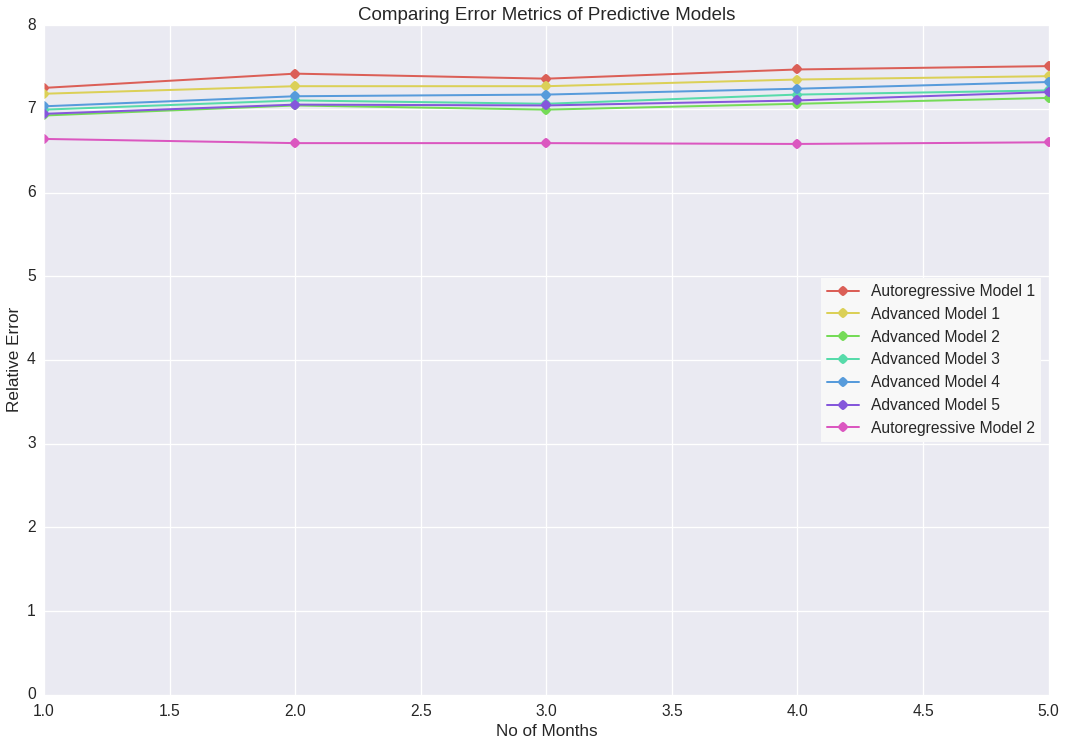
\includegraphics[width=\textwidth]{ModelComparison_Oil.png}
\caption{Relative performance of the Autoregressive model, ARMA model and the Autoregressive model incorporating macroeconomic factors predicting the price of oil}
\label{fig:ModelComparison_Oil.png}
\end{figure}

\begin{figure}
\centering
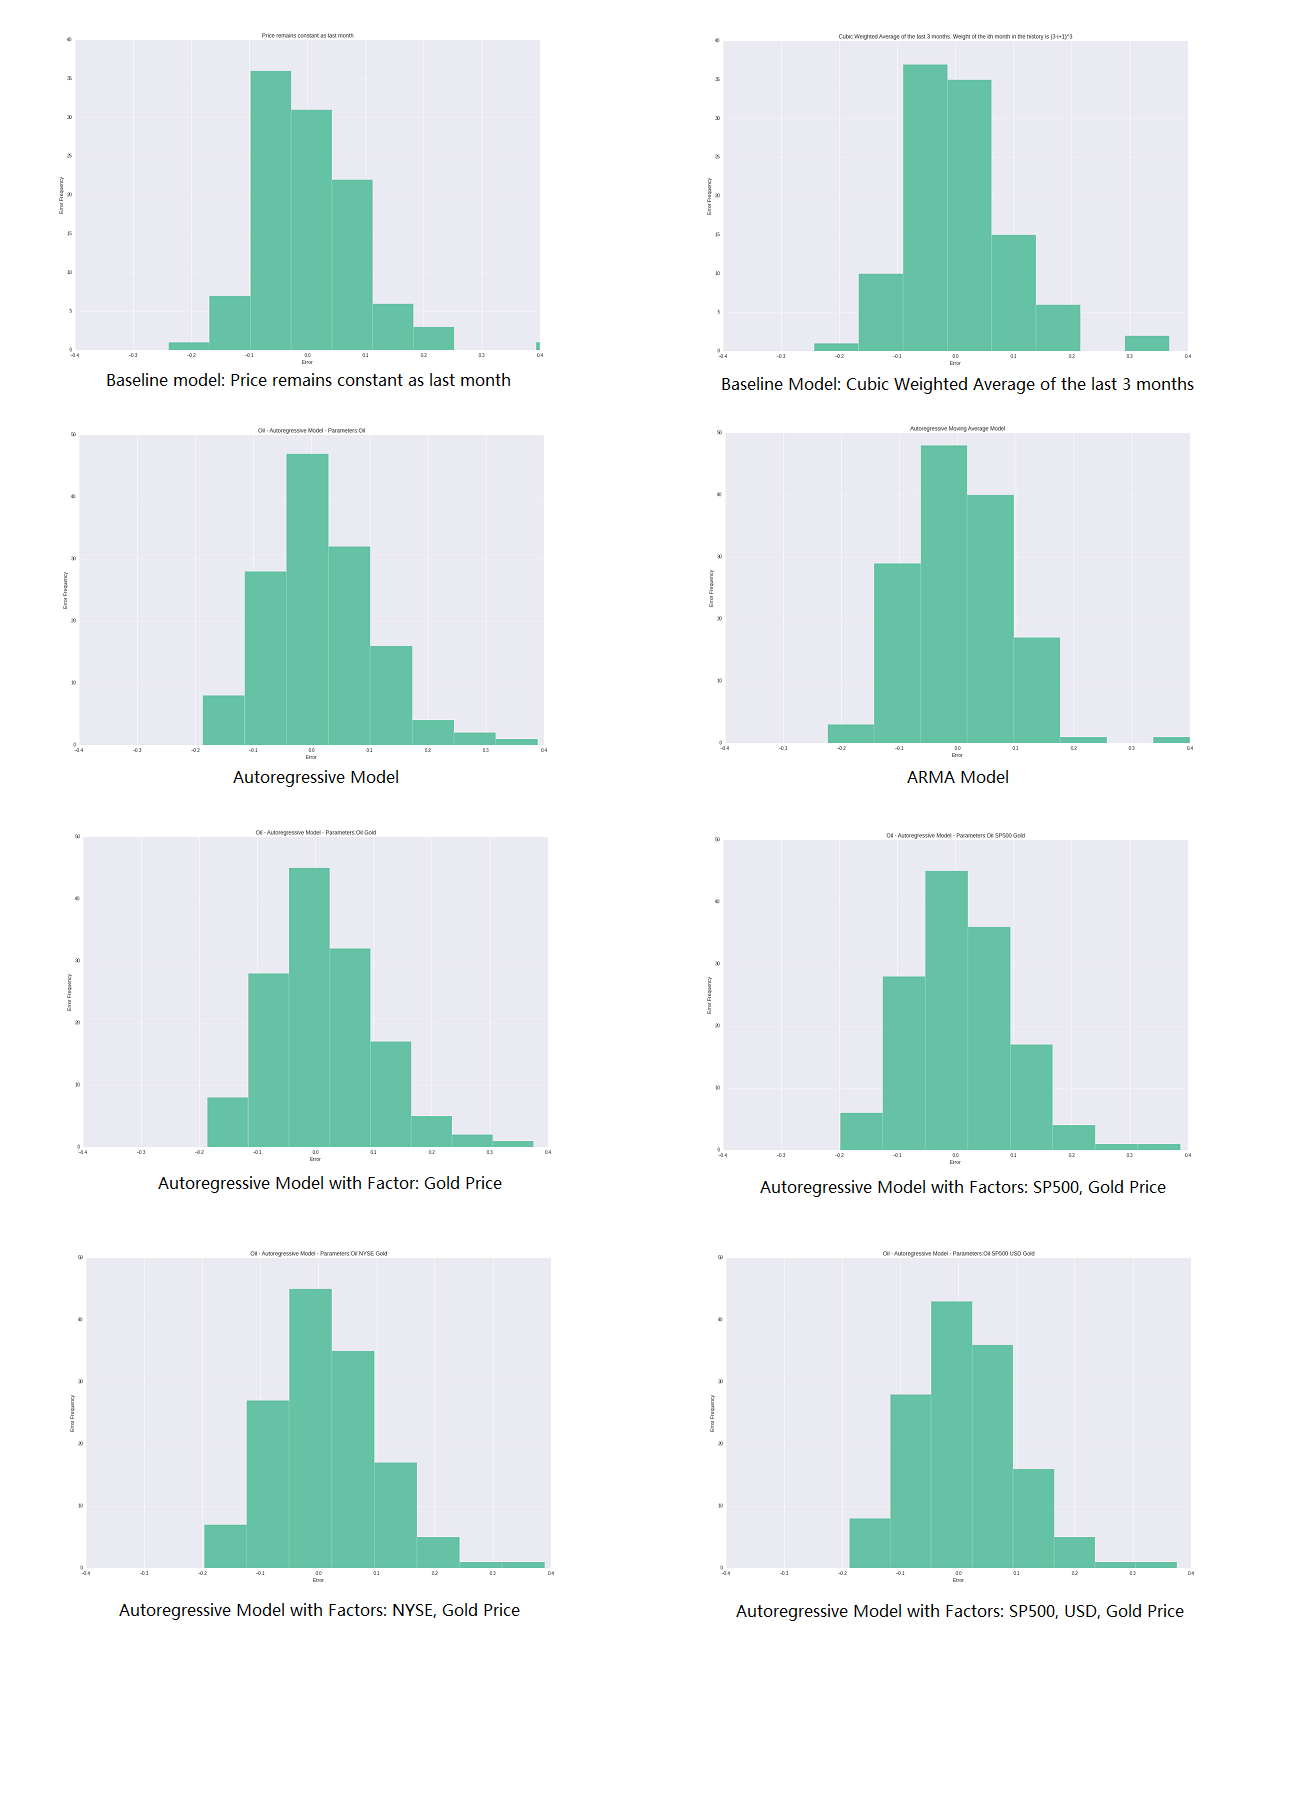
\includegraphics[width=\textwidth]{OilErrorHistogram.png}
\caption{Error histograms of models predicting the price of oil}
\label{fig:OilErrorHistogram.png}
\end{figure}

\newpage

\subsection{Performance of Models Predicting the Price of Gold}

\noindent The following is a summary of all the models used for predicting the price of gold \\
 
\begin{table}
\begin{center}
\begin{tabular}{|c|c|c|c|c|c}
\hline
\textbf{Model} & \textbf{Mean Rel Error} & \textbf{Mean Abs Error} & \textbf{RMSE} \\ \hline \hline
$ Baseline\ - Price\ Remains\ Same$ & $4.61\%$ & $56.11$ & $75.36$  \\ \hline
$ Baseline\ - Price\ is\ a\ Weighted\ Average$ & $4.56\%$ & $55.78$ & $73.27$ \\ \hline \hline
$ Autoregressive\ Model $  & $4.24\%$ & $46.61$ & $65.91$ \\ \hline
$ Autoregressive\ Moving\ Average\ Model $ & $4.32\%$ & $45.73$ & $63.71$ \\ \hline \hline
$ Autoregressive-factors:\ CSI $ & $4.24\%$ & $46.62$ & $65.87$ \\ \hline
$ Autoregressive-factors:\ CSI,\ Oil $ & $4.3\%$ & $47.24$ & $65.86$ \\ \hline
$ Autoregressive-factors:\ SP500,\ NYSE,\ Oil $ & $4.68\%$ & $49.17$ & $65.67$ \\ \hline
$ Autoregressive-factors:\ SP500,\ NYSE,\ CSI,\ Oil $ & $5.61\%$ & $55.02$ & $69.51$ \\ \hline \hline
$ Futures\ Prices\ Model\ 1 $ & $2.34\%$ & $26.86$ & $35.42$ \\ \hline
$ Futures\ Prices\ Model\ 2 $ & $4.03\%$ & $42.71$ & $79.49$ \\ \hline
\end{tabular}
\end{center} 

\caption{Error metrics of various models predicting the price of gold.}
\end{table} 


\subsubsection{Summary}

\begin {itemize}

\item Among the autoregressive models, the pure autoregressive model considering only historical gold prices performed the best with a Mean Relative Error of 4.24\%. It performs better than both the baseline models. \\
\item Among the multiple linear regressive models considering economic factors, the model considering CSI as a factor performed best with a Mean Relative Error of 4.24\%. This model also performed better compared to the Baseline Model 1 and 2. It performs as good as the pure autoregressive model. \\
\item Models considering other combinations of economic factors fail to perform better than the pure autoregressive model.\\
\item Overall, the Futures Models 1, with a Mean Relative Error of 2.34\% perform significantly better (almost twice as good) as compared to any of the autoregressive or multiple linear regressive models. \\
\item Futures Model 2, which considers the difference between spot and futures prices, does not perform better than the Futures Model 1.

\end {itemize}


\autoref{fig:ModelComparison_Gold.png} shows the comparison of the relative errors of different predictive models. \autoref{fig:GoldErrorHistogram.png} shows the error histograms generated by different models.

\begin{figure}
\centering
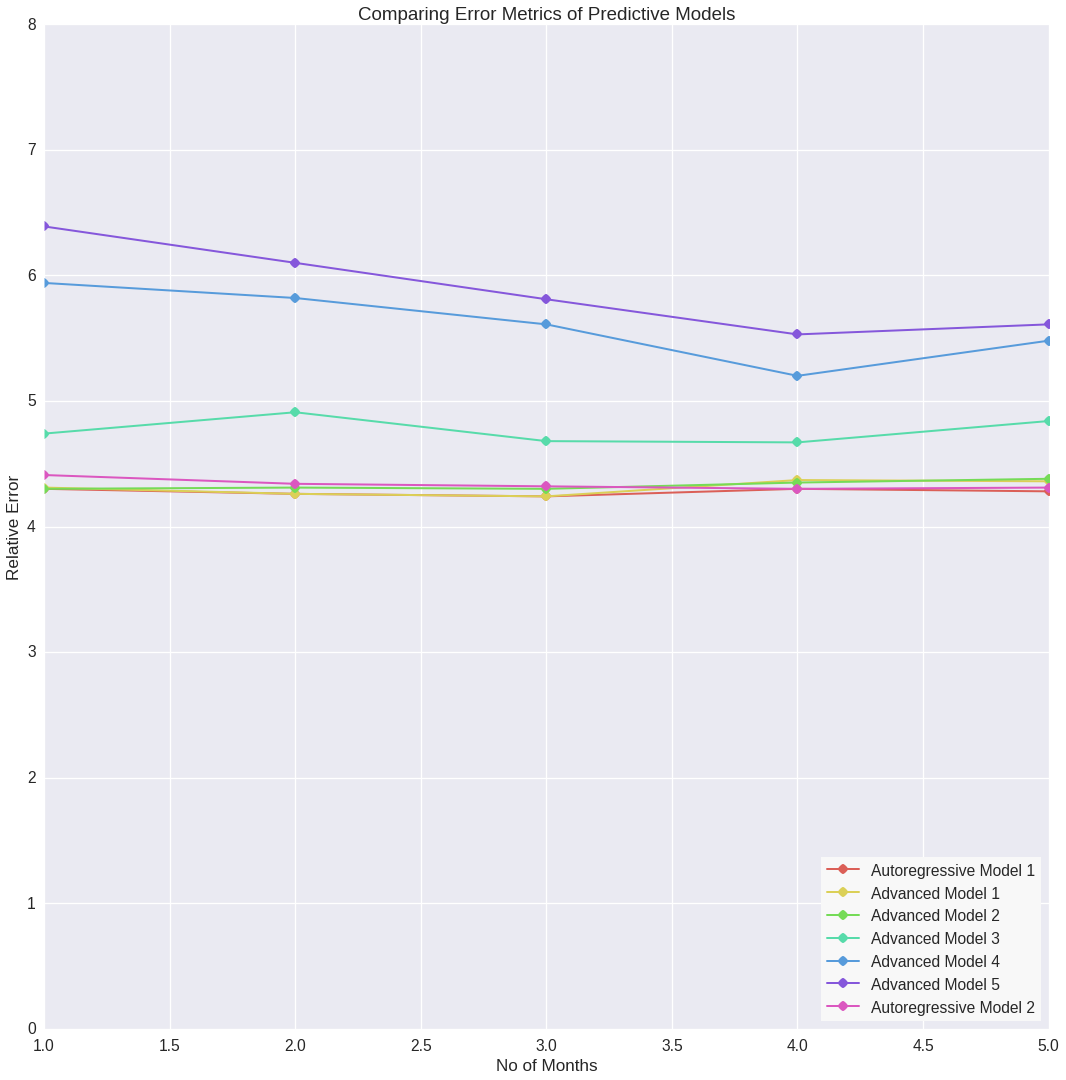
\includegraphics[width=\textwidth]{ModelComparison_Gold.png}
\caption{Relative performance of the Autoregressive model, ARMA model and the Autoregressive model incorporating macroeconomic factors predicting the price of gold}
\label{fig:ModelComparison_Gold.png}
\end{figure}

\begin{figure}
\centering
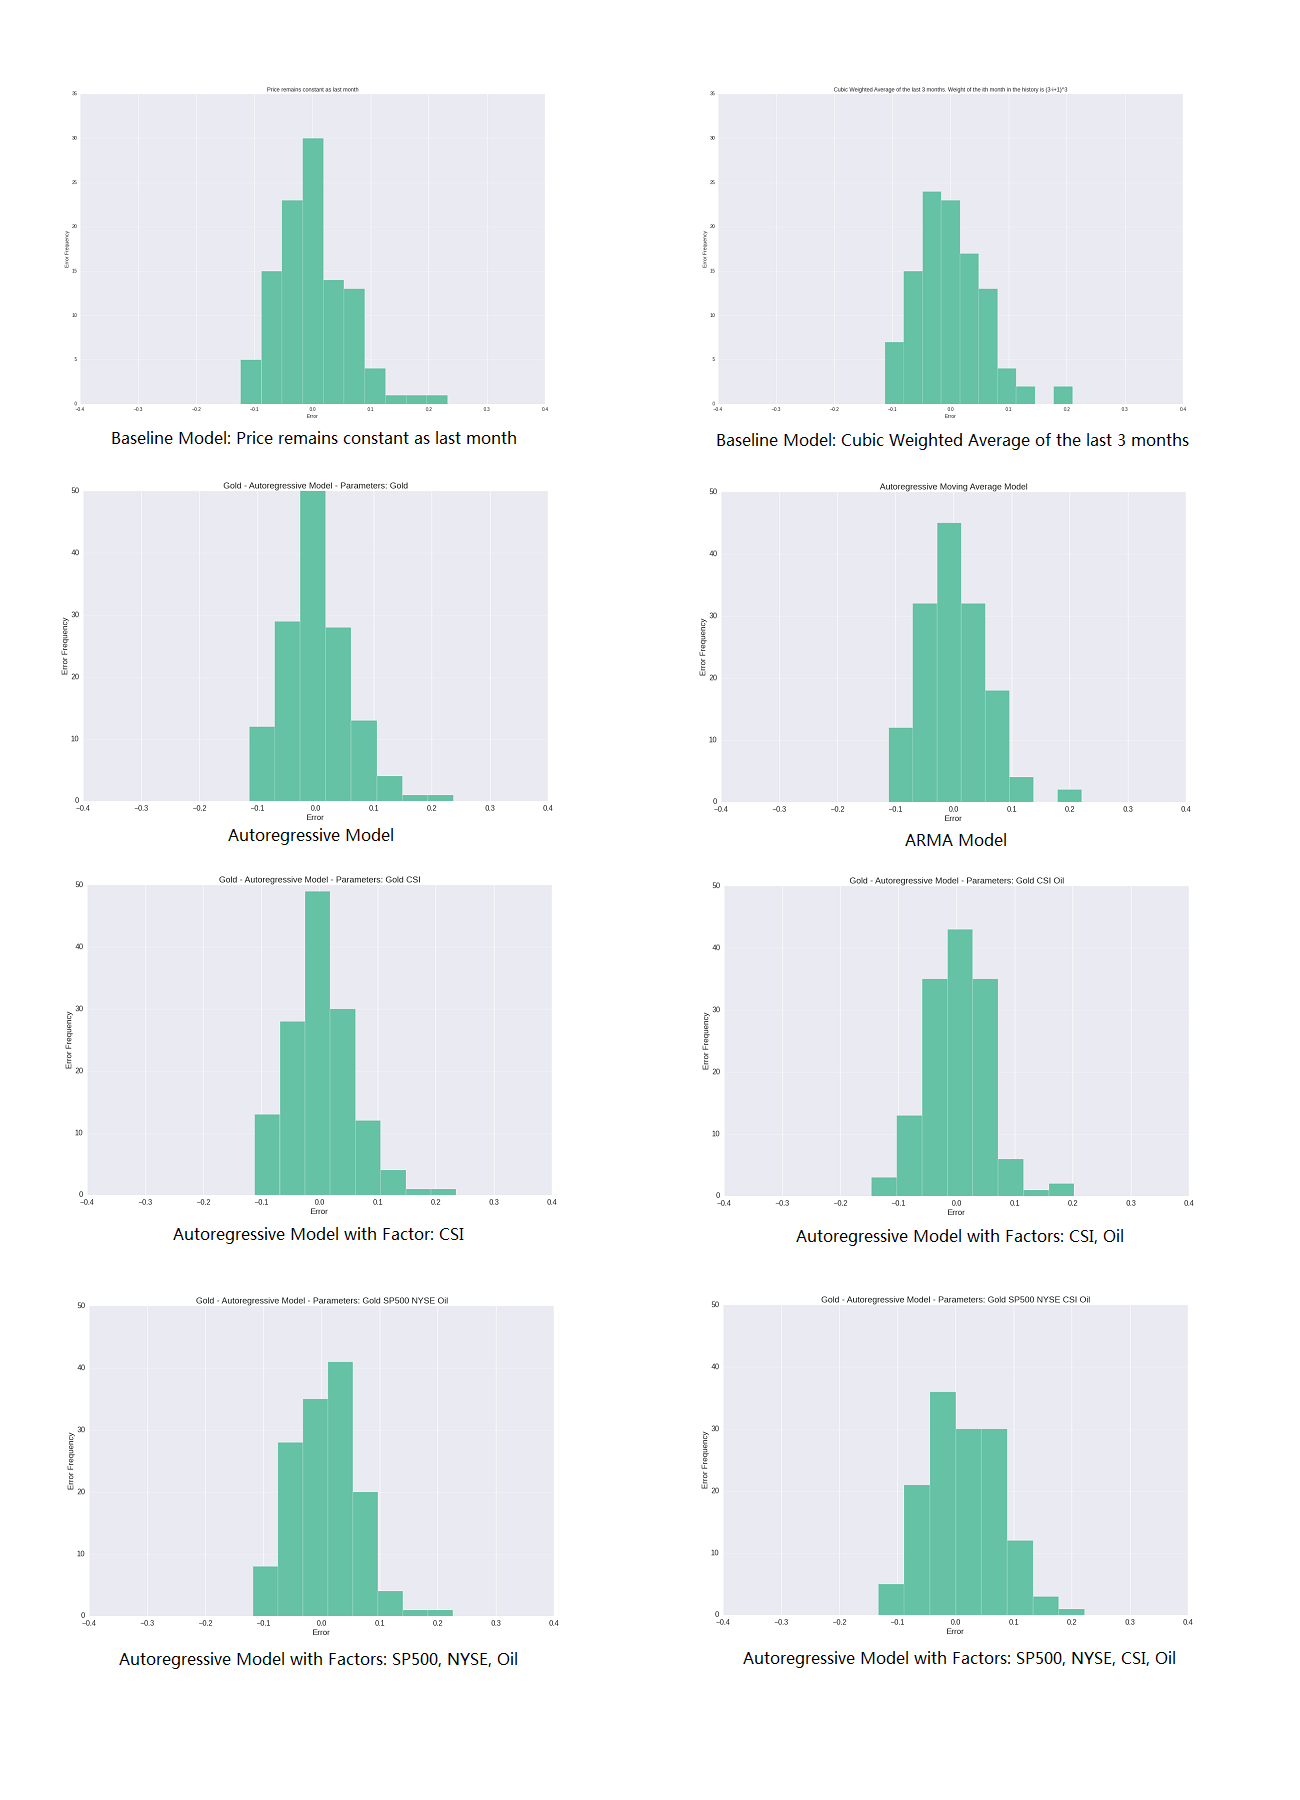
\includegraphics[width=\textwidth]{GoldErrorHistogram.png}
\caption{Error histograms of models predicting the price of gold}
\label{fig:GoldErrorHistogram.png}
\end{figure}


\newpage
\section{Final Prediction and Conclusions}
\subsection {Final Prediction}
\noindent The predicted price of WTI Crude Oil on Jan 1, 2015 as of Dec 1, 2014 is \\
\textbf{63.30 USD per Barrel} \\

\noindent The predicted price of Gold on Jan 1, 2015 as of Dec 1, 2014 is \\
\textbf{1179.25 USD per ounce} \\

\subsection {Difficulties We Had to Overcome in Building Good Models and Investigations for Subsequent Groups}

\begin{itemize}

\item \textbf{Missing Data} \\
We initially faced a problem of missing data rows in the data sets of certain economic parameters. This resulted in a dimension mismatch error while merging multiple time series into a single data frame. Using an inner join to combine data frames resolved our issue. \\

\item \textbf{Inflation Adjustment} \\
The data we used for our predictions were monetary time series, and it is important to inflation adjust the data before performing a correlation. We initially had not adjusted for inflation, which resulted in very high correlation between the oil/gold price and related macroeconomic factors. Most of this correlation was meaningless and could be attributed to inflation. \\

Adjusting the data for inflation reduced the correlation to a large extent, and also resulted in an improvement in our models. Earlier, the performance of models incorporating economic factors was worse compared to all other models. Adjusting for inflation resulted these models performing better than the baseline and the pure autoregressive models. This is definitely an indicator that highly correlated factors are not always the best predictors. \\

\item \textbf{Data Unavailability} \\
We intended to include more macroeconomic factors into our model, but certain factors could not be included due to the unavailability of historical data. For instance, Euro-USD exchange rate was a factor we failed to incorporate because the Euro was introduced only in 1992, and we were using past 30 years data (since 1986) for the other factors.  \\

\item \textbf{Downloading Futures Data} \\
The futures data is available as individual files for every month of the year. Downloading approximately 360 files, and reading them into a single data frame was a challenge. 

\item \textbf{Outliers in Futures Data} \\
The futures model was giving us an RMSE >13, which was a very high number compared to the other models. However, the mean error and variance were not as bad. We had almost disregarded this model assuming that it wasn't good enough. \\

But when we plotted the error histogram, we noticed an outlier. Most of the errors were lying between -0.1 and +0.1, but this outlier had an error of -0.9 which was causing the large RMSE. When we investigated the data set, we found that the outlier was caused due to a data entry being 0. We then removed the outlier from our data sets, we realized that the futures model was by far the best model we had developed. \\

The important lesson we learnt was that we should always plot graphs to detect outliers, and it is important to know the reason behind the outlier. Also, since a RMS amplifies the error, we shouldn't simply disregard the results. Instead, we should look deeper into the data and investigate the cause. 
\end{itemize}



\subsubsection*{Acknowledgments.} Dr. Steven Skiena. Professor Keli (Andrew) Xiao.


\begin{thebibliography}{4}
\bibitem{opec} "OPEC : Home.". \url{http://www.opec.org/}

\bibitem{eiafactors} "Energy and Financial Markets: What Drives Crude Oil Prices". \url{http://www.eia.gov/finance/markets}

\bibitem{oildollar} Zhang, Yue-Jun, et al. "Spillover effect of US dollar exchange rate on oil prices." Journal of Policy Modeling 30.6 (2008): 973-991.

\bibitem{gold-shafiee} Shahriar Shafiee,  Erkan Topal.:An overview of global gold market and gold price forecasting. ScienceDirect. Volume 35, Issue 3, September 2010, 178--189 (2010)

\bibitem{gold-zhang} Zhang, Yue-Jun, and Yi-Ming Wei. "The crude oil market and the gold market: Evidence for cointegration, causality and price discovery." Resources Policy 35.3 (2010): 168-177.

\bibitem{oil-zhang}Zhang, Xun, Kin Keung Lai, and Shou-Yang Wang. "A new approach for crude oil price analysis based on empirical mode decomposition." Energy Economics 30.3 (2008): 905-918.

\bibitem{gold-Ismail}Z. Ismail, A. Yahya and A. Shabri. "Forecasting Gold Prices Using Multiple Linear Regression Method." American Journal of Applied Sciences 6 (8) (2009): 1509-1514.

\bibitem{gold-url1} The Relationship between Gold and Crude Oil Price, \url{http://www.marketoracle.co.uk/Article38141.html}

\bibitem{csi-1} What's the difference between consumer confidence and consumer sentiment?, \url{http://www.investopedia.com/ask/answers/09/consumer-confidence-sentiment-difference.asp}

\bibitem{csi-1} What's the difference between consumer confidence and consumer sentiment?, \url{http://www.investopedia.com/ask/answers/09/consumer-confidence-sentiment-difference.asp}

\bibitem{csi-2} Consumer confidence index, \url{http://en.wikipedia.org/wiki/Consumer_confidence_index}

\bibitem{engle} Engle, Robert. "GARCH 101: The use of ARCH/GARCH models in applied econometrics." Journal of economic perspectives (2001): 157-168.

\bibitem{gold-pso}Hadavandi, Esmaeil, Arash Ghanbari, and Salman Abbasian-Naghneh. "Developing a Time Series Model Based on Particle Swarm Optimization for Gold Price Forecasting." Business Intelligence and Financial Engineering (BIFE), 2010 Third International Conference on. IEEE, 2010.

\bibitem{gold-ref1}Khashei, Mehdi, Mehdi Bijari, and Gholam Ali Raissi Ardali. "Improvement of auto-regressive integrated moving average models using fuzzy logic and artificial neural networks (ANNs)." Neurocomputing 72.4 (2009): 956-967.

\bibitem{gold-ref2}Khashei, Mehdi, Seyed Reza Hejazi, and Mehdi Bijari. "A new hybrid artificial neural networks and fuzzy regression model for time series forecasting." Fuzzy Sets and Systems 159.7 (2008): 769-786.

\bibitem{huntington} Huntington, Hillard G. "Oil price forecasting in the 1980s: what went wrong?." The Energy Journal (1994): 1-22.

\bibitem{pindyck} Pindyck, Robert S. "The long-run evolution of energy prices." The Energy Journal (1999): 1-27.

\bibitem{dongbing}Dong, Bing, Cheng Cao, and Siew Eang Lee. "Applying support vector machines to predict building energy consumption in tropical region." Energy and Buildings 37.5 (2005): 545-553.

\bibitem{yang} Yang, C. W., Ming-Jeng Hwang, and Bwo-Nung Huang. "An analysis of factors affecting price volatility of the US oil market." Energy Economics 24.2 (2002): 107-119.

\bibitem{quandal} Quandl - Find, Use and Share Numerical Data. \url{https://www.quandl.com}

\bibitem{csi}\url{http://future.aae.wisc.edu/data/monthly_values/by_area/998?grid=true}

\end{thebibliography}

\end{document}
